\chapter{Hardware -- konfiguracja}
Ten rozdział poświęcony jest dokładnemu opisowi konfiguracji układu elektronicznego mikrokontrolera i~jego peryferiów oraz procesu generowania kodu w~C. Autor wyszczególnia kluczowe decyzje konfiguracyjne i~uzasadnia podjęte wybory. Autor przytacza fragmenty dokumentacji płytki ewaluacyjnej, instrukcji obsługi użytkownika oraz innych dokumentów dostarczonych przez producenta mikrokontrolera, aby poprzeć wywody i~obliczenia obecne w~tym rozdziale. Całość procesu dobierania parametrów i~ustawień komponentów płytki ewaluacyjnej przeprowadzona jest we wspomnianym w~sekcji \ref{sec:IDE} środowisku STM32CubeMX. Zastosowano podejście bare-metal programming, by w~jak największym stopniu ograniczyć narzuty czasowe operacji niezwiązanych ściśle z~przetwarzaniem dźwięku.
\section{Obliczeniowa platforma sprzętowa}
Jak już opisano wcześniej, do realizacji projektu autor wybrał mikrokontroler na płytce ewaluacyjnej NUCLEO-STM32F446RE. Płytka posiada 64 piny GPIO (General Purpose Input Output) do zastosowania na różnorodne sposoby -- do komunikacji ze światem zewnętrznym. Centralnym elementem płytki jest mikrokontroler z~procesorem ARM Cortex M4 w~architekturze 32-bit RISC\footnote{Przetwarzanie Danych przez Ograniczoną Listę Rozkazów (ang. Reduced Instruction Set Computing)}. Mikroprocesor pracuje z~częstotliwością zegara równą \SI{180}{\MHz} i~posiada 512~KB pamięci flash oraz 128~KB pamięci SRAM\footnote{Pamięć SRAM pozwala na bezpośredni zapis i~odczyt danych wewnątrz rejestrów procesora bez oczekiwania na dane. W~tym urządzeniu działa podobnie do pamięci cache procesora.}.
\section{Konfiguracja peryferiów}
\label{sec:configuration}
Konfigurację systemu należy rozpocząć od uruchomienia wszystkich wymienionych wcześniej elementów cyfrowych. Dobór parametrów omówiony zostanie po kolei dla każdego komponentu:
\begin{itemize}
	\item Przetwornik analogowo-cyfrowy nr 1 (od głównego mikrofonu)\\
	Oba przetworniki skonfigurowane są w~trybie dualnym jednoczesnej konwersji zwykłej\footnote{Ang. Dual regular simultaneous mode}. Pozwala to na synchronizowane działanie komponentów z~przetwornikiem numer~1~jako elementem nadrzędnym. Sygnał z~mikrofonu kierowany jest do zerowego kanału tego przetwornika. Częstotliwość pracy przetworników uzależniona jest od napięcia zasilania, co oznacza, że przy dostarczonym napięciu \SI{3.3}{\V} komponenty pracują z~częstotliwością w~przybliżeniu równą \SI{30}{\MHz}. Konwersja wywoływana jest przez sygnał zegarowy timera~3~magistrali mikrokontrolera, odmierzający interwał czasowy równy \SI{100}{\micro\s}, aby zapewnić stały krok próbkowania. Oprócz tego preskaler przetwornika powoduje 4-krotne zmniejszenie częstotliwości pracy, aby spowolnić jego działanie i~przez to zwiększyć dokładność pomiaru. Czas próbkowania ustawiony jest na 3~cykle, co w~połączeniu ze stałym czasem konwersji, równym 12 cykli \cite{RM0390}, daje 15 cykli składających się na pojedynczą konwersję sygnału. Oznacza to, że przy wspomnianej wcześniej częstotliwości pracy, jedna konwersja zajmować będzie w~przybliżeniu:
		
\begin{center}
		$ T_{przetwarzania} = \frac{preskaler \cdot (t_{probkowania} + t_{konwersji})}{f_{pracy\_adc}} = \frac{4\cdot(3+12)}{\SI{30}{\MHz}} = \SI{2}{\micro\s} $
	
	$ f_{przetwarzania} = \frac{1}{T_{przetwarzania}} = \frac{1}{\SI{0.000002}{\s}} \approx \SI{500}{\kHz} $ 
	
\end{center}
	W~związku z~tym, przetwornik w~takiej konfiguracji mógłby efektywnie konwertować sygnały o~górnej granicznej częstotliwości widma równej \SI{250}{\kHz}. Należy jednak wziąć pod uwagę fakt, że sygnały audio słyszalne dla człowieka zawierają się w~zakresie od około \SI{20}{\Hz} do około \SI{20000}{\Hz}, co oznacza, że należy znacznie ograniczyć częstotliwość pracy układu. Dodatkowo, sygnały które zazwyczaj tłumi się aktywnie, zajmują dolną część pasma częstotliwościowego, zatem można jeszcze bardziej ograniczyć tę częstotliwość próbkowania. Ostatecznie wybrano częstotliwość próbkowania równą \SI{10}{\kHz} (okres próbkowania równy \SI{100}{\micro\s}). Takie ograniczenie osiągnięto biorąc pod uwagę czas, jaki zajmują obliczenia generujące sygnał przeciwstawny, częstotliwość wzbudzeń pochodzących od timera oraz czas konwersji DAC. Wszystkie te oraz inne czynniki składają się na zmniejszenie efektywnej zdolności przetwarzania układu. Głównym czynnikiem motywującym wybór krótkiego czasu próbkowania (zamknięcia klucza S\&H) jest konieczność zminimalizowania elektronicznego narzutu czasowego wykonanych operacji. Czas, jaki zajmą wszystkie operacje układu, nie może przekroczyć czasu, który fali akustycznej zajmuje przebycie drogi od pierwszego mikrofonu do drugiego. Przekroczenie tej granicy spowodowałoby drastyczne ograniczenie skuteczności urządzenia -- odpowiedź filtra byłaby spóźniona i~co najwyżej powielałaby hałas.
	\item Przetwornik analogowo-cyfrowy nr 2 (od mikrofonu odsłuchowego)\\
	Ten przetwornik jest podrzędny względem pierwszego, co oznacza, że synchronizuje się z~nim i~dostosowuje swoje działanie do wspólnego transferu danych poprzez DMA w~trybie~2. Ten tryb opisany jest dokładniej w~punkcie dotyczącym konfiguracji kontrolera DMA. Sygnał kierowany jest do pierwszego kanału tego przetwornika.
	\item Timer~3\\
	Ten komponent skonfigurowano tak, by odmierzał interwał czasowy równy \SI{100}{\micro\s}. Oznacza to, że pomimo częstotliwości, jaką daje przetwornik, narzucona zostaje częstotliwość próbkowania równa \SI{10}{\kHz}, co daje częstotliwość Nyquista równą \SI{5}{\kHz}. Licznik ten taktowany jest magistralą APB1 o~częstotliwości \SI{84}{\MHz}, co oznacza, że przy pomocy preskalera oraz rejestru odmierzającego należało obniżyć częstotliwość wzbudzeń tego licznika właśnie na wspomniane wyżej \SI{10}{\kHz}. Ponadto, gdy znana jest już górna granica częstotliwościowa filtra, można dobrać parametry analogowych filtrów antyaliasingowych, które zapobiegają zakłócaniu pracy urządzenia przez nieobsługiwane ,,wysokie'' częstotliwości.
	\item Przetwornik cyfrowo-analogowy\\
	Ten komponent, w~przeciwieństwie do poprzedniego, nie posiada tak wiele opcji konfiguracyjnych. Wybrano tutaj transfer jednokanałowy, gdyż układ emitował będzie sygnał monofoniczny. Gdyby układ miał spełniać funkcję słuchawek stereo z~dwoma kanałami, można byłoby wtedy otworzyć drugi kanał tego przetwornika. Ponieważ nie wybrano żadnego trybu wyzwalacza, konwersja następuje automatycznie po upłynięciu jednego cyklu zegara APB1 (o~częstotliwości \SI{84}{\MHz}) od momentu wpisania nowej wartości do odpowiedniego rejestru.
	\item Kontroler DMA nr~1\\
	Kontroler użyty jest do transferu wartości wag filtra LMS z~pamięci urządzenia do kontrolera UART, który następnie wysyła te dane do komputera walidującego. Akcja ta wykonywana jest tylko raz, po wzbudzeniu przez testera poprzez wciśnięcie przycisku lub wysłanie przez UART komendy '0' (co zatrzymuje algorytm i~wysyła przerwanie wywołujące transfer danych). Wystarczy więc odpowiednio zmodyfikować funkcję obsługującą przerwanie przychodzącej transmisji UART oraz drugą, odpowiadającą za obsługę przerwania zewnętrznego wzbudzenia na wyprowadzeniach GPIO, aby otrzymać zapisane w~pamięci nastawy algorytmu.
	\item Kontroler DMA nr~2\\
	Ten element jest konieczny do prawidłowego funkcjonowania przetworników ADC w~trybie dualnym. Gdy przetworniki skończą konwersję, 12-bitowe wyniki tego działania zapisywane są do zmiennych 16-bitowych, które następnie łączone są w~jedną zmienną 32-bitową (bity wyników zapisywane są w~tej zmiennej w~kolejności: dane z~ADC2, a~następnie dane z~ADC1). Taka pojedyncza zmienna 32-bitowa jest następnie transferowana przez kontroler DMA do pamięci mikrokontrolera, skąd należy wyłuskać pojedyncze wyniki konwersji. Jest to charakterystyczne zachowanie przetworników ADC w~trybie dualnym przy współpracy z~kontrolerem DMA. To właśnie ten specyficzny tryb podawania danych do DMA jest nazywany trybem~2, co może być nieco mylące i~sugerować, że jest to tryb kontrolera, mimo iż jest to tak naprawdę tryb przetworników.
	\item USART (Universal Synchronous/Asynchronous Receiver/Transmitter)\\
	W~przypadku tego komponentu wybrano transmisję asynchroniczną z~szybkością transmisji równą 115200~bitów na sekundę. Długość pojedynczej wysyłanej danej ustawiono na 8~bitów. Zrezygnowano z~bitu parzystości. Następnie, po stronie komputera PC odbierającego te dane, ustawiono takie same parametry kontrolera UART i~włączono tryb odczytu danych typu float. Pozwala to na bezpośredni odczyt wartości wysłanych nastaw (rys. \ref{fig:realterm}). Te dane następnie są używane w~pakiecie obliczeniowym MATLAB, by na ich podstawie zbadać odpowiedź impulsową filtra.
	\begin{figure}[h!]
		\centering
		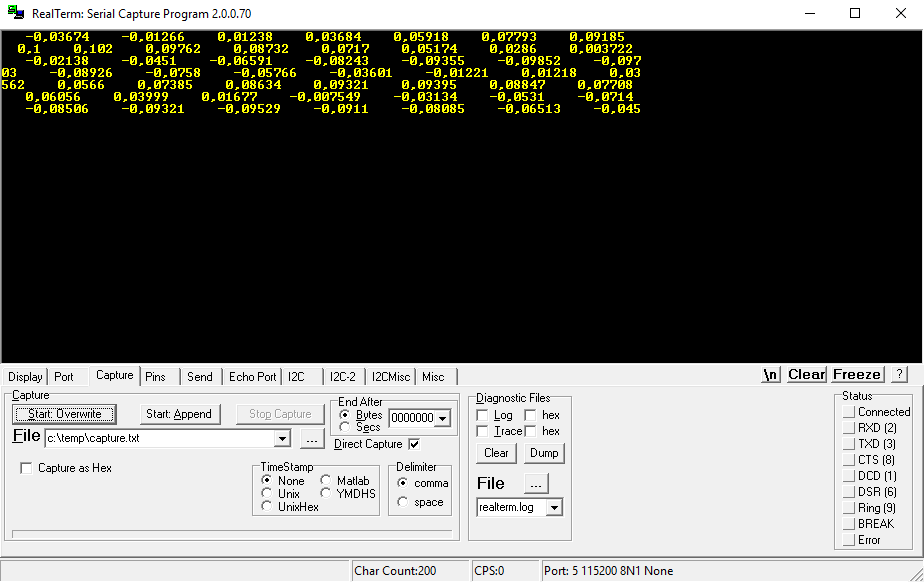
\includegraphics[scale=0.5]{../Assets/RealTerm.png}
		\caption{Wagi filtra LMS dla jednego z~przypadków testowych odebrane poprzez port szeregowy przy użyciu programu RealTerm.}
		\label{fig:realterm}
	\end{figure}
\end{itemize}
\section{Wygenerowanie kodu w języku C}
\label{sec:configGenerate}
Ustawienia poczynione w~programie STM32CubeMX zapamiętywane są w~pliku o~formacie .ioc, który okazuje się być zapisem tekstowym poszczególnych ustawień wraz z~przypisaniem wartości i~trybów. Plik ten jest interpretowany przez STM32CubeMX i~na jego podstawie generowana jest konfiguracja (wraz z~ukazującym ją interfejsem graficznym). Po przeprowadzeniu konfiguracji układu oraz sprawdzeniu ustawień zegarów i~liczników mikrokontrolera, można przystąpić do wygenerowania kodu konfiguracyjnego w~języku~C. Program użyty do konfiguracji pozwala na wygenerowanie współpracującego z~biblioteką HAL (użytą przez autora do zaimplementowania całości programu) kodu podzielonego na fragmenty automatycznie generowane oraz sekcje użytkownika. Jest to o~tyle istotne, że w~przypadku wystąpienia potrzeby zmiany konfiguracji któregoś komponentu, ponowne wygenerowanie kodu konfiguracyjnego nie ingeruje w~specjalne sekcje użytkownika. Pozwala to jeszcze sprawniej prototypować układy bez obawy o~utratę wypracowanych efektów. Poza wspomnianą funkcjonalnością, STM32CubeMX wspiera również generowanie kodu w~konwencjach specyficznych dla poszczególnych środowisk programistycznych -- można wybrać jedno z~nich z~listy dostępnej w~zakładce ,,Project~Manager''. Autor wybrał środowisko SW4STM32, czyli wspomniany w~rozdziale 3 i~użyty w~implementacji ,,System Workbench for STM32''. Moduł generowania kodu dostarcza jeszcze kilku zaawansowanych narzędzi i~ustawień, jednak autor nie zmieniał ich automatycznie dobranych parametrów.